\documentclass[addpoints]{exam}
\usepackage[utf8]{inputenc}
\usepackage[portuguese]{babel}
\usepackage[LGRgreek]{mathastext}
\usepackage{graphicx,graphics}
\usepackage{hyperref}
%\usepackage{framed}
\usepackage{multirow}
\usepackage{booktabs}
\usepackage{pdfpages} 

\footer{}{\thepage}{}

%%% INÍCIO DOS COMANDOS ACRESCENTADOS NO NETBOOK %%%%%%%%%%%%%%%%%%%
\newcommand*{\renameenviron}[1]{%
  \expandafter\let\csname exam-#1\expandafter\endcsname
      \csname #1\endcsname
  \expandafter\let\csname endexam-#1\expandafter\endcsname
      \csname end#1\endcsname
  \expandafter\let\csname #1\endcsname\relax
  \expandafter\let\csname end#1\endcsname\relax
}
\renameenviron{framed}
\renameenviron{shaded}
\renameenviron{leftbar}
%%% FIM DOS COMANDOS ACRESCENTADOS NO NETBOOK %%%%%%%%%%%%%%%%%%%
\usepackage{framed}

\renewcommand{\arraystretch}{1.3}
%\setlength{\tabcolsep}{pt}
 
\pointpoints{ponto}{pontos}
\bonuspointpoints{ponto extra}{pontos extra}
 
\totalformat{Pregunta \thequestion: \totalpoints pontos}
 
\chqword{Pregunta}
\chpgword{Página}
\chpword{Pontos}
\chbpword{Pontos extra}
\chsword{Pontos obtidos}
\chtword{Total}

\hqword{Questão}
\hpgword{Página}
\hpword{Pontos}
\hsword{Pontos obtidos}
\htword{Total}

 
\begin{document}
 
\large

\begin{center}
\Large
\textbf{Laboratório de Eletrônica Básica II – EE641}
\end{center}

\large
\vspace{2mm}

\noindent\textbf{Profs.:} Dr. Eduardo T. Costa\hfill \textbf{Turma 01/2022} \\
\textbf{PED:} Mathias Scroccaro Costa \hfill %\textbf{e-mail:} mathias.scroccaro@gmail.com

\normalsize
 
\vspace{5mm}
 

 
\noindent\makebox[0.72\textwidth]{Nome: \enspace\hrulefill}
\hfill
\makebox[0.2\textwidth]{RA: \enspace\hrulefill}

\vspace{5mm}

\noindent\makebox[0.72\textwidth]{Nome: \enspace\hrulefill}
\hfill
\makebox[0.2\textwidth]{RA: \enspace\hrulefill}

\vspace{5mm}

\noindent\makebox[0.72\textwidth]{Nome: \enspace\hrulefill}
\hfill
\makebox[0.2\textwidth]{RA: \enspace\hrulefill}


%\begin{center}
%\gradetable[h][questions]
%\end{center}

\vspace{2mm}


\begin{center}
\large
\textbf{FILTRO SALLEN-KEY}
\normalsize
\end{center}

\begin{questions}

\section*{Filtro Sallen-Key}

\question \label{part:circuito} Complete o circuito de amplificação e processamento de sinais de ECG acrescentando o filtro ativo de segunda ordem sallen-key, à direita do nó ``Vout'', conforme mostra o esquemático da Figura \ref{cir:1}. Utilize R = 11 k$\Omega$ e C = 100 nF. Continue soldando os componentes na \textbf{placa furada padrão}. Não esqueça de disponibilizar \textit{pinheads} machos, para a alocação de \textit{mini jumpers}, pois serão fundamentais ao testar o circuito.

\begin{figure}[h!]
\begin{center}
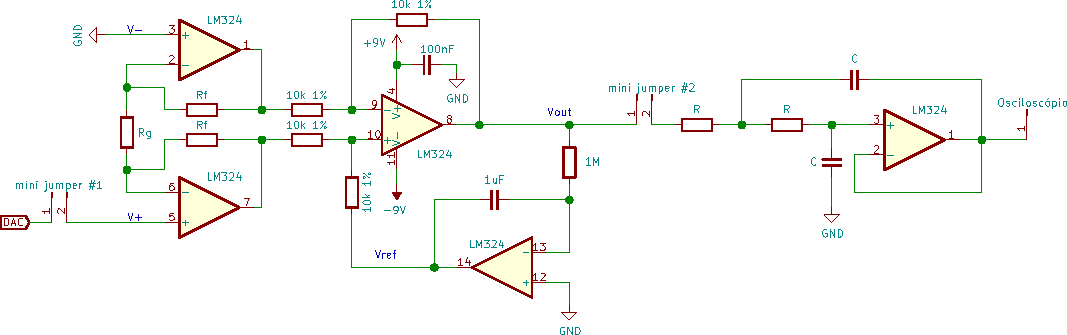
\includegraphics[width=\textwidth]{imagens/complete_circuit.pdf}
\end{center}
\caption{Circuito amplificador de instrumentação e filtro Sallen-Key.}
\label{cir:1}
\end{figure}

\pagebreak

\begin{parts}

\part Verifique a funcionalidade, banda de passagem e frequência de corte do filtro montado. Descreva o método utilizado e acrescente imagens do osciloscópio, mostrando suas constatações. 

\pagebreak

\section*{Apresentação do projeto final}

\part Desenvolva um programa para Arduino que exiba formas de onda dos sinais de ECG disponibilizados via Moodle, intercaladas por um período de 3 s. Grave seu programa no microcontrolador e o conecte ao circuito desenvolvido. Verifique as formas de onda na saída do filtro. Tome todos os devidos cuidados ao realizar as conexões e procedimentos! \textit{Sempre monitore a corrente da fonte de alimentação}, para intervir em eventuais não conformidades. Imprima e anexe as formas de onda verificadas. Anexe ao relatório o código-fonte desenvolvido.

\pagebreak

\end{parts}

\question (PÓS EXPERIMENTO) Explique o funcionamento de todo o circuito de geração e captação de sinais de ECG.

\begin{framed}
\vspace{19cm}
\end{framed}


\end{questions}

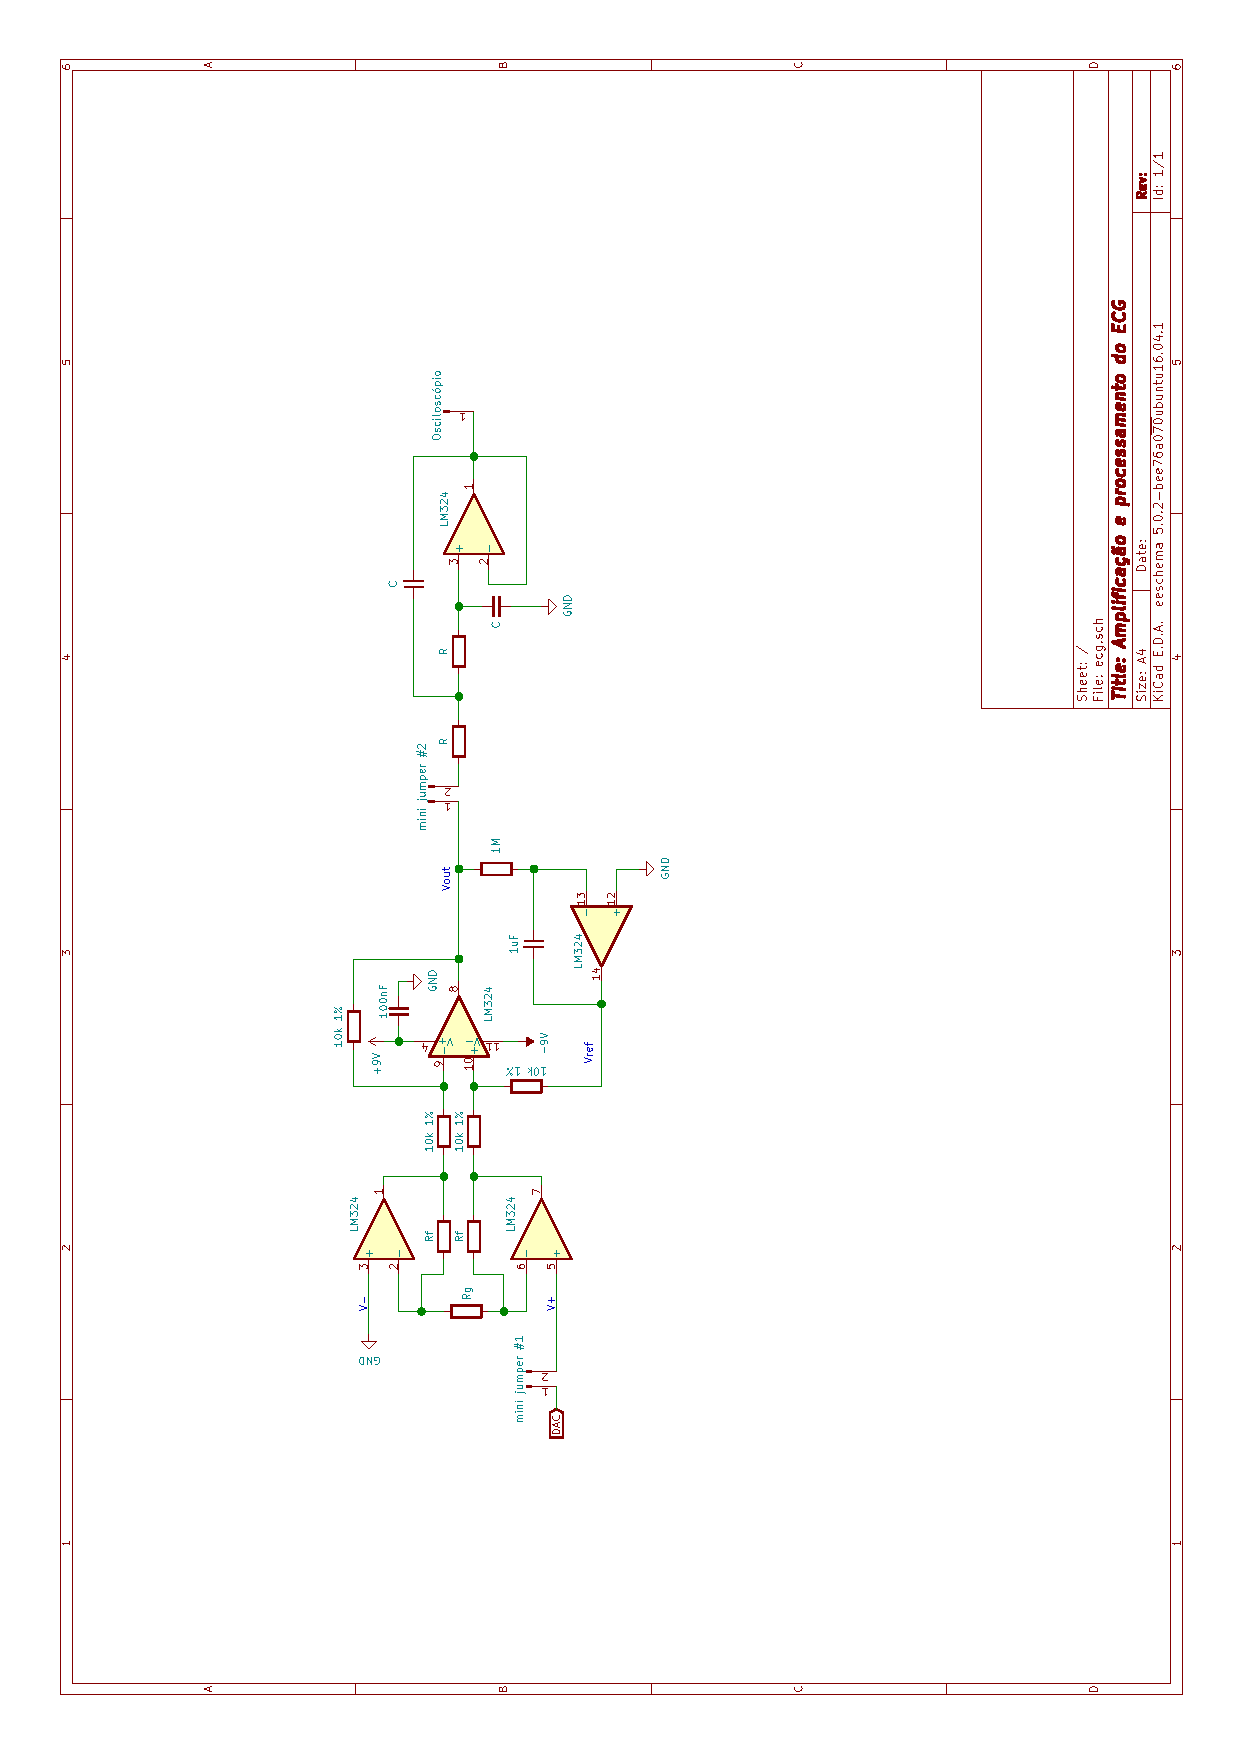
\includepdf[page={1}]{imagens/ecg.pdf}

\end{document}
